\documentclass[../Main.tex]{subfiles}
\setcounter{chapter}{14}

\begin{document}
\phantomsection
\chapter{L15: Modules}
Consider the vector space $\R^n \coloneqq \{(a_1,\dots,a_n)\mid a_i \in \R, \, i=1,2,\dots,n\}$. We know from our experiences in linear algebra that addition is defined as
\[\begin{array}{c}
	\vec{v} = (v_1,\dots,v_n)\\
	\vec{w} = (w_1,\dots,w_n)
\end{array}\implies \vec{v}+\vec{w} \coloneqq (v_1+w_1,\dots,v_n+w_n)\in \R^n\] 
\begin{figure*}[!h]
	\centering
	\includegraphics[width=0.5\textwidth]{VecAdd2}
\end{figure*}

\Note $(\R^n,+) $ is an abelian (commutative) group with addition:
\begin{itemize}
	\item (Additive identity) $\exists \vec{0} \in \R^n$ such that $\vec{0} + \vv = \vv + \vec{0} = \vv \quad \forall \vv \in \R^n$
	\item (Associative) $(\vv +\vw) + \vu = \vv + (\vw + \vu) \quad \forall \vv,\vw,\vu \in \R^n$
	\item (Additive inverse) $\forall \vv \in \R^n, \exists\,\, \text{-}\vv \in \R^n$ such that $\vv + (-\vv) = (-\vv ) + \vv = \vec{0}$
	\item (Abelian) $\vv + \vw = \vw + \vv \quad \forall \vv,\vw \in \R^n$ 
\end{itemize}
$\R^n$ also has \textbf{scalar multiplication}: If $a\in \R$ and $\vv \in \R^n$ then
\[a\rdot \vv = (av_1,av_2,\dots,av_n) \in \R^n \]
We can think of scalar multiplication as a map
\begin{align*}
\R \times \R^n &\to \R^n\\
(a,\vv)&\mapsto a\rdot \vv
\end{align*}
Suppose $a,b\in \R$ and $\vv,\vw \in \R^n$, then scalar multiplication has the following properties
\begin{enumerate}[label=(\arabic*)]
	\item $(a+b)\rdot \vv = a\rdot \vv + b\rdot \vv$
	\item $(ab)\rdot \vv = a\rdot (b\rdot \vv)$
	\item $a\rdot (\vv + \vw) = a\rdot \vv + a \rdot \vw$
	\item $1\rdot \vv = \vv$
\end{enumerate}
\begin{dfn}[title = \texorpdfstring{$R$}{R}-module]
	Let $R$ be a ring.\\
	A \textbf{(left) module over }$R$ or ($R$-\textbf{module}) is a set $M$ with
	\begin{enumerate}[label=(\arabic*)]
		\item a binary operation $+$ such that $(M,+)$ is an Abelian group,
		\item an action of $R$ on $M$ i.e a map
		\begin{align*}
		R\times M &\to M \\
		(r,m) &\mapsto r\rdot m
		\end{align*}
	\end{enumerate}
	such that for $r,s\in R$ and $m,n\in M$
	\begin{enumerate}[label=(\roman*)]
		\item $(r+s)\rdot m = r\rdot m + s\rdot m$
		\item $(rs)\rdot m = r\rdot (s\rdot m)$
		\item $r\rdot (m+n) = r\rdot m + r\rdot n$
		\item If $1 \in R$ then $1 \rdot m = m$ and the module is called \textbf{Unital}.
	\end{enumerate}
\end{dfn}
\Note We can define a \textbf{right} $R$-module by $m\rdot r$ with scalar multiplication on the right.The only difference is associativity being $m\rdot (rs) = (m\rdot r)\rdot s$. Contrast this to property (ii) which says the action of $rs$ on $m$ is the action of $s$ first and then acting by $r$ , whereas now, it is the action of $r$ first then acting by $s$ and these two notions coincide only when $R$ is commutative. \textbf{We will always be talking about left $R$-modules unless explicitly stated}\\
\Note If $R$ is a commutative ring then any left $R$-module has a natural right $R$-module structure as well:
\[(rs)\rdot m = (sr)\rdot m \longleftrightarrow m\rdot (sr) = m\rdot (rs) = (m\rdot r)\rdot s\]
\begin{dfn}[title =  \texorpdfstring{$F$}{F}-vector space]
	If $F$ is a field, then we refer to $F$-modules as $F$-\textbf{vector spaces}. In this sense $\R^n$ is an $\R$-vector space.
\end{dfn}
\Obs If $R\subset S$ is as subring and $M$ is an $S$-module then $M$ is also a $R$-module by restricting scalar multiplication to $R$. For example, $\C^2$ is a $\C$-vector space but it is also an $\R$-vector space. \\
If $a\in \R,\, \vv = (v_1,v_2)\in \C^2$ then $a\rdot \vv = (av_1,av_2)\in \C^2$ still makes sense.
\begin{example}
	For any ring $R$, consider
	\[R^n \coloneqq \{(a_1,\dots,a_n)\mid a_i\in R, \, i=1,2,\dots,n\}\]
	with component-wise addition 
	\[(a_1,a_2,\dots,a_n)+(b_1,b_2,\dots,b_n) \coloneqq (a_1+b_1,a_2+b_2,\dots,a_n+b_n)\]
	\Exr $(R^n,+)$ is an abelian group.\\
	Scalar multiplication is also component-wise, for $a\in R$ and $(a_1,\dots,a_n)\in R^n$, defined as
	\[a\rdot (a_1,\dots,a_n)\coloneqq (a\rdot a_1,\dots,a\rdot a_n)\]
	\Exr $(R^n,+)$ is an $R$-module with this scalar multiplication.\\
	This is called the \textbf{free $R$-Module of rank $n$}.
\end{example}
\begin{example}
	The \textbf{trivial module} $0\coloneqq \{\vec{0}\}$ which has $\forall r \in R, \, r\rdot \vec{0} \coloneqq \vec{0}$.
\end{example}
\begin{example}
	Any ideal of a ring $I\subset R$ is an $R$-module with scalar multiplication as  ring multiplication:
	\begin{align*}
	R \times I &\to I\\
	(r,a) &\mapsto ra
	\end{align*}
\end{example}
\begin{example}
	Quotient rings of $R$ are $R$-modules with scalar multiplication as ring multiplication:
	\begin{align*}
	R\times R/I &\to R/I\\
	(r,\bar{a}) &\mapsto \obar{r\rdot a}
	\end{align*}
	\Exr Module property (ii) $(rs)\rdot \bar{a}=r\rdot (s\rdot \bar{a})$ holds.
\end{example}
Recall a vector subspace $W\subset \R^n$ is a subset such that
\begin{enumerate}[label = (\roman*)]
	\item $\vw_1+\vw_2 \in W, \quad \forall \vw_1, \vw_2 \in W$
	\item $\vec{0}\in W$
	\item $a\rdot \vw \in W, \quad \forall a \in \R, \,\vw \in W$
	\item $-\vw \in W, \quad \forall \vw \in W$
\end{enumerate}
\begin{example}
	$\R^2$ has subspaces $\vec{0},\R^2,\Span \left\{\begin{pmatrix}
	a\\b
	\end{pmatrix} \mid a,b\in \R\right\}$
	\begin{figure*}[!h]
		\centering
		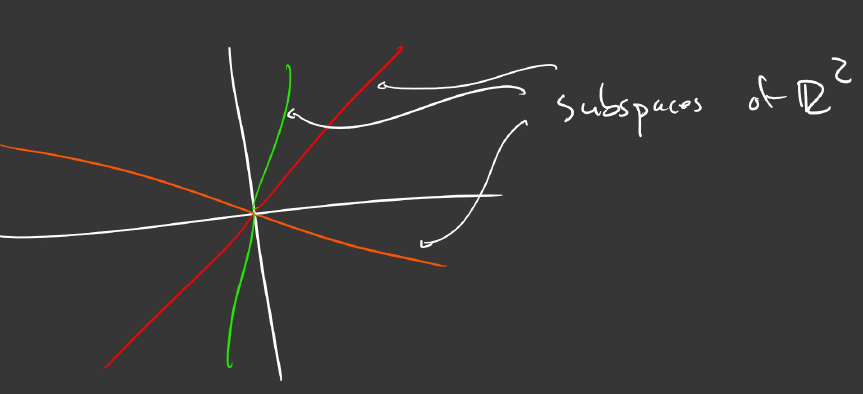
\includegraphics[width=0.5\textwidth]{Subspace}
	\end{figure*}
\end{example}
\begin{dfn}[title = {Submodule, Subspace}]
	A \textbf{submodule} of an $R$-module $M$ is a subgroup $N\subset M$ such that it is closed under scalar multiplication, i.e for all $r\in R, n\in N, r\rdot n\in N$.\\
	If $F$ is a field, we call $F$-submodules \textbf{$F$-subspaces}
\end{dfn}
\begin{example}
	Every module is a submodule of itself.
\end{example}
\begin{example}
	Every module has the $0$-module.
\end{example}
\begin{example}
	If we think about a ring $R$ as a module over itself, then the submodules of $R$ are the ideals of $R$.\\
	\Note The only subspaces of $\R$ are $0$ or $\R$ (since the only ideals in a field are $0$ and the field itself).
\end{example}
\begin{example}
	$\Z$-\textbf{modules}.\\
	Let $M$ be any abelian group. Define for all $n\in \Z$ and $a\in M$,
	\[
	n\rdot a \coloneqq \begin{cases}
	\underbrace{a+a+a+\dots+a}_{n\text{-times}} & n> 0 \\
	0 & n = 0 \\
	\underbrace{(-a)+(-a)+(-a)+\dots+(-a)}_{(-n)\text{-times}} & n <0
	\end{cases}
	\]
	\Exr $(n+m)\rdot a=n\rdot a+m\rdot a$ and $(nm)\rdot a=n\rdot (m\rdot a)$\\
	This is a common sense way to come up with a $\Z$-module structure on any abelian group and
	so $\{\Z\text{-modules}\}= \{\text{Abelian groups}\}$ For example $\modZ{4}$ is a $\Z$-module as
	\[n\rdot \obar{0}=\obar{0},\quad n\rdot \obar{1}=\obar{n},\quad n\rdot \obar{2}=\obar{2n},\quad n\rdot \obar{3}=\obar{3n}\]
\end{example}
We can then immediately think of a large list of $\Z$-modules: $\Z^n$ for $n\ge 1$ and $\modZ{n}$ for $n\ge 2$.
\begin{example}
	$(\modZ{n})$-\textbf{module}\\
	Let $M$ be a $(\modZ{n})$-module. \\
	Then 
	\begin{align*}
	&\underbrace{(1+1+1+\dots+1)}_{n\text{-times}}\rdot a = 0\rdot a = 0 \quad \forall a \in M\\
	=&\underbrace{1\rdot a+1\rdot a+1\rdot a+\dots+1\rdot a}_{n\text{-times}}\\
	=&\underbrace{a+a+a+\dots+a}_{n\text{-times}}
	\end{align*}
	So in a $\modZ{n}$-module, the sum of any element with itself $n$ times is going to be equal to 0.
	For example $\modZ{2}$ is a $(\modZ{4})$-module because $1$ added to itself four times is $0$ as seen
	\[\underbrace{(1\,\mathrm{mod}\,2) + (1\,\mathrm{mod}\,2)}_{0\,\mathrm{mod}\,2} + \underbrace{(1\,\mathrm{mod}\,2)+ (1\,\mathrm{mod}\,2)}_{0 \,\mathrm{mod}\,2} = 0\,\mathrm{mod}\,2\]
\end{example}
A \textbf{linear transformation}  $T\colon \R^n \to \R^m$ is a map between two vector spaces such that
\begin{align*}
T(\vv+\vw)&=T\vv+T\vw\\
T(a\vv)&=a\rdot T\vv
\end{align*}
As an example,
\begin{align*}
T\colon \R^3&\to \R^2 \\
(x,y,z)&\mapsto (2x+y-z,x+2y)
\end{align*}
which, recall, we can represent as a matrix 
\[\begin{pmatrix}
2&1&-1\\
1&2&0
\end{pmatrix}\begin{pmatrix}
x\\y\\z
\end{pmatrix}=\begin{pmatrix}
2x+y-z\\x+2y
\end{pmatrix}\]
\begin{dfn}[title = {\texorpdfstring{$R$}{R}-module homomorphism, \texorpdfstring{$F$}{F}-linear transformation}]
	Let $R$ be a ring and $M,N$ be $R$-modules.\\
	An \textbf{$R$-module homomorphism} from $M$ to $N$ is a map $f\colon M\to N$ such that
	\begin{enumerate}[label=(\arabic*)]
		\item $f(m+n)=f(m)+f(n)\quad \forall m,n\in M$
		\item $f(a\rdot m) = a\rdot f(m) \quad \forall a \in R, m\in M$
	\end{enumerate}
	If $F$ is a field, we call $F$-module homomorphisms \textbf{$F$-linear transformations}.
\end{dfn}
\end{document}